\documentclass[varwidth=\maxdimen, border=5pt]{standalone}

% Diamond Model of Intrusion Analysis
%   - https://apps.dtic.mil/sti/pdfs/ADA586960.pdf
%   - https://www.recordedfuture.com/blog/diamond-model-intrusion-analysis
%   - FOR578 (2025), Book 1, Page 79
%   - FOR578 (2025), Book 2, Page 28

\usepackage[utf8]{inputenc}
\usepackage[T1]{fontenc}
\usepackage{tikz}
\usepackage{enumitem}
\usepackage{varwidth}
\usepackage[none]{hyphenat}
\usetikzlibrary{positioning, calc}

% vertex item environment with hanging indent if line break occurs
\newcommand{\vitem}[1]{\raggedright \leftskip=1em \parindent=-1em #1\par}

% activity name label, including optional tracking ID
\newcommand{\namelabel}[2][]{%
  #2%
  \ifx\relax#1\relax\else
    \\[2pt]{\normalsize\upshape (#1)}%
  \fi
}

\begin{document}

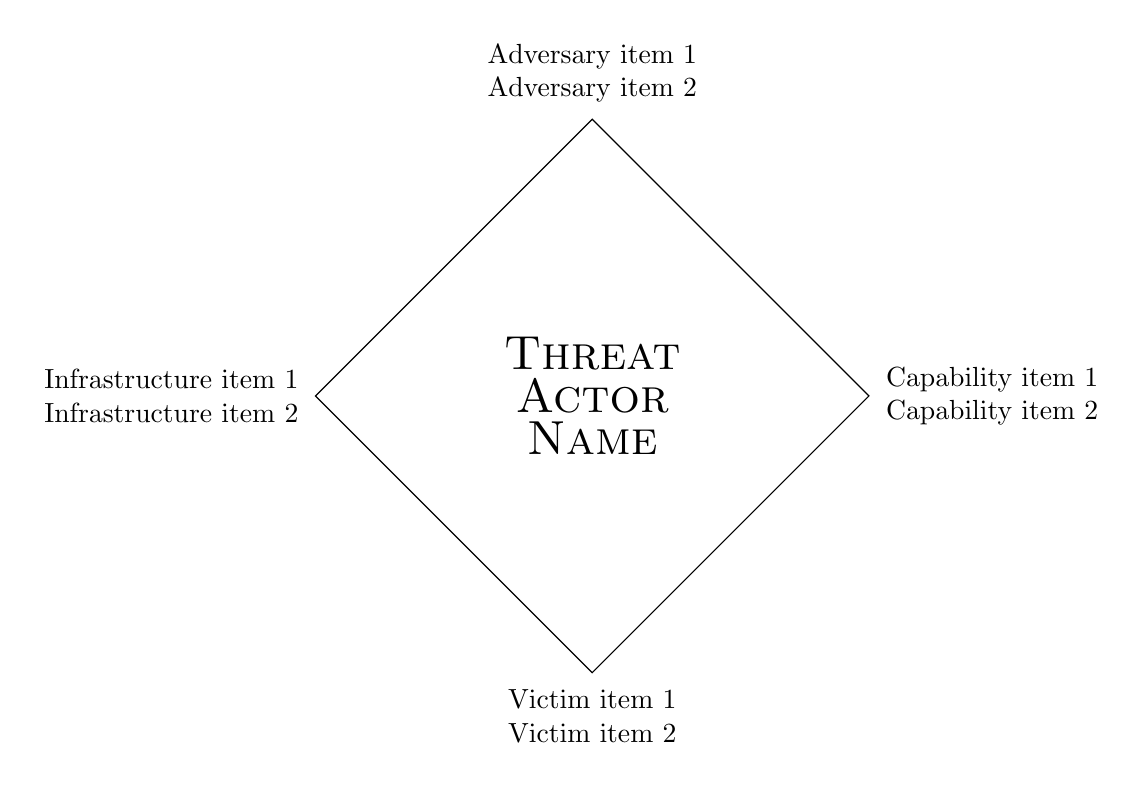
\begin{tikzpicture}[
  node distance=10em,
  name label/.style={
    align=center,
    text width=9em,
    font=\LARGE\scshape\linespread{0.7}\selectfont,
  },
  vertex list/.style={
    inner sep=6pt,
    execute at begin node=\begin{varwidth}{12em}\raggedright,
    execute at end node=\end{varwidth},
  },
]

\coordinate (core) at (0, 0);

% Central label
\node[name label] at (core) {\namelabel{Threat Actor Name}};

% Vertex labels
\node[vertex list, above=of core, anchor=south] (adversary) {
  \vitem{Adversary item 1}
  \vitem{Adversary item 2}
};
\node[vertex list, right=of core, anchor=west] (capability) {  % or TTP
  \vitem{Capability item 1}
  \vitem{Capability item 2}
};
\node[vertex list, below=of core, anchor=north] (victim) {
  \vitem{Victim item 1}
  \vitem{Victim item 2}
};
\node[vertex list, left=of core, anchor=east] (infrastructure) {
  \vitem{Infrastructure item 1}
  \vitem{Infrastructure item 2}
};

% Draw diamond
\draw (adversary.south) -- (capability.west) -- (victim.north) -- (infrastructure.east) -- cycle;

% Make the left/right extent symmetric so the diamond is centred in the output
%\path let \p1=(infrastructure.west), \p2=(capability.east), \p3=(adversary.north), \p4=(victim.south),
%  \n1={max(-\x1,\x2)} in
%  [use as bounding box] (-\n1,\y4) rectangle (\n1,\y3);

\end{tikzpicture}

\end{document}